\hypertarget{cmd:extras-standard}{}
\section{Standardlayouts erstellen und bearbeiten}
\label{sec:templates}
Um nicht jeden Plot einzeln formatieren zu m�ssen, k�nnen auch Standardlayouts erstellt
werden, die dann relativ einfach auf neue Plots �bertragen werden k�nnen. W�hlen Sie hierzu
\menu{Extras / Standard} (Abb. \ref{fig:standardeinstellungen}).
Wenn Sie einen neuen Standard erzeugen m�chten, w�hlen Sie \ctrl{Hinzuf�gen}. Es
erscheinen zwei Editierfelder, in denen Sie zum einen nach Klicken in das Einstellungen-Feld
(links) einen Namen f�r Ihr Layout vergeben k�nnen (z.B. LfW-Querprofil) und zum anderen
einen Stempel zuordnen k�nnen. Sobald Sie in das Stempelfeld klicken erscheint ein
Listenfeld mit allen verf�gbaren Stempeln. Wenn Sie eine Standardeinstellung markieren und
anschlie�end \ctrl{Bearbeiten} dr�cken, kommen Sie wieder zum Dialogfeld \dialog{Eigenschaften}.
Hier k�nnen Sie s�mtliche Einstellungen wie unter \ref{sec:profildarstellung}
erl�utert selektieren und dem Standard zuordnen. Beim sp�teren �ffnen eines neuen
Plots / Profils wird als Default der Standard gew�hlt, dessen Kontrollk�stchen aktiv geschaltet
wurde. Es besteht auch die M�glichkeit keinen Standard vorzudefinieren (alle K�stchen
ausgeschaltet). Um einem einzelnen Plot einen Standard zuzuordnen w�hlen Sie in der Karte
\dialog{Allgemein} unter \ctrl{Einstellungen / Eigenschaften} das gew�nschte Layout aus.

\begin{figure}[h]
	\begin{center}
		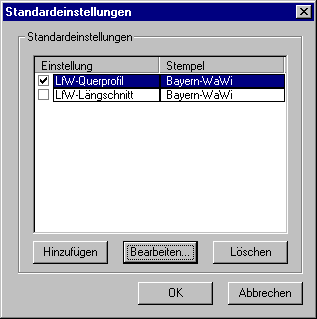
\includegraphics[scale=0.80]{standardeinstellungen}
	\end{center}
	\caption{Standardeinstellungen}
	\label{fig:standardeinstellungen}
\end{figure}
